%\documentclass{beamer}
\documentclass[aspectratio=169]{beamer}
\usetheme{Boadilla}

%\usetheme{Warsaw}
%\setbeamercovered{transparent}
\beamertemplatetransparentcoveredhigh
\usepackage[portuges]{babel}
\usepackage[latin1]{inputenc}
\usepackage{lmodern}
\usepackage[T1]{fontenc}
\usepackage{hyperref} 
\usepackage[portuguese, linesnumbered, vlined, titlenumbered, ruled]{algorithm2e}

\newcommand{\eng}[1]{\textsl{#1}}
\newcommand{\cod}[1]{\texttt{#1}}

\title[Apresenta��o]{Curso Intelig�ncia Artificial: do Zero ao Infinito}
\author[Frederico Oliveira]{Data Augmentation}
\institute[UFMT]{Universidade Federal de Mato Grosso}
\date{}
%\titlegraphic{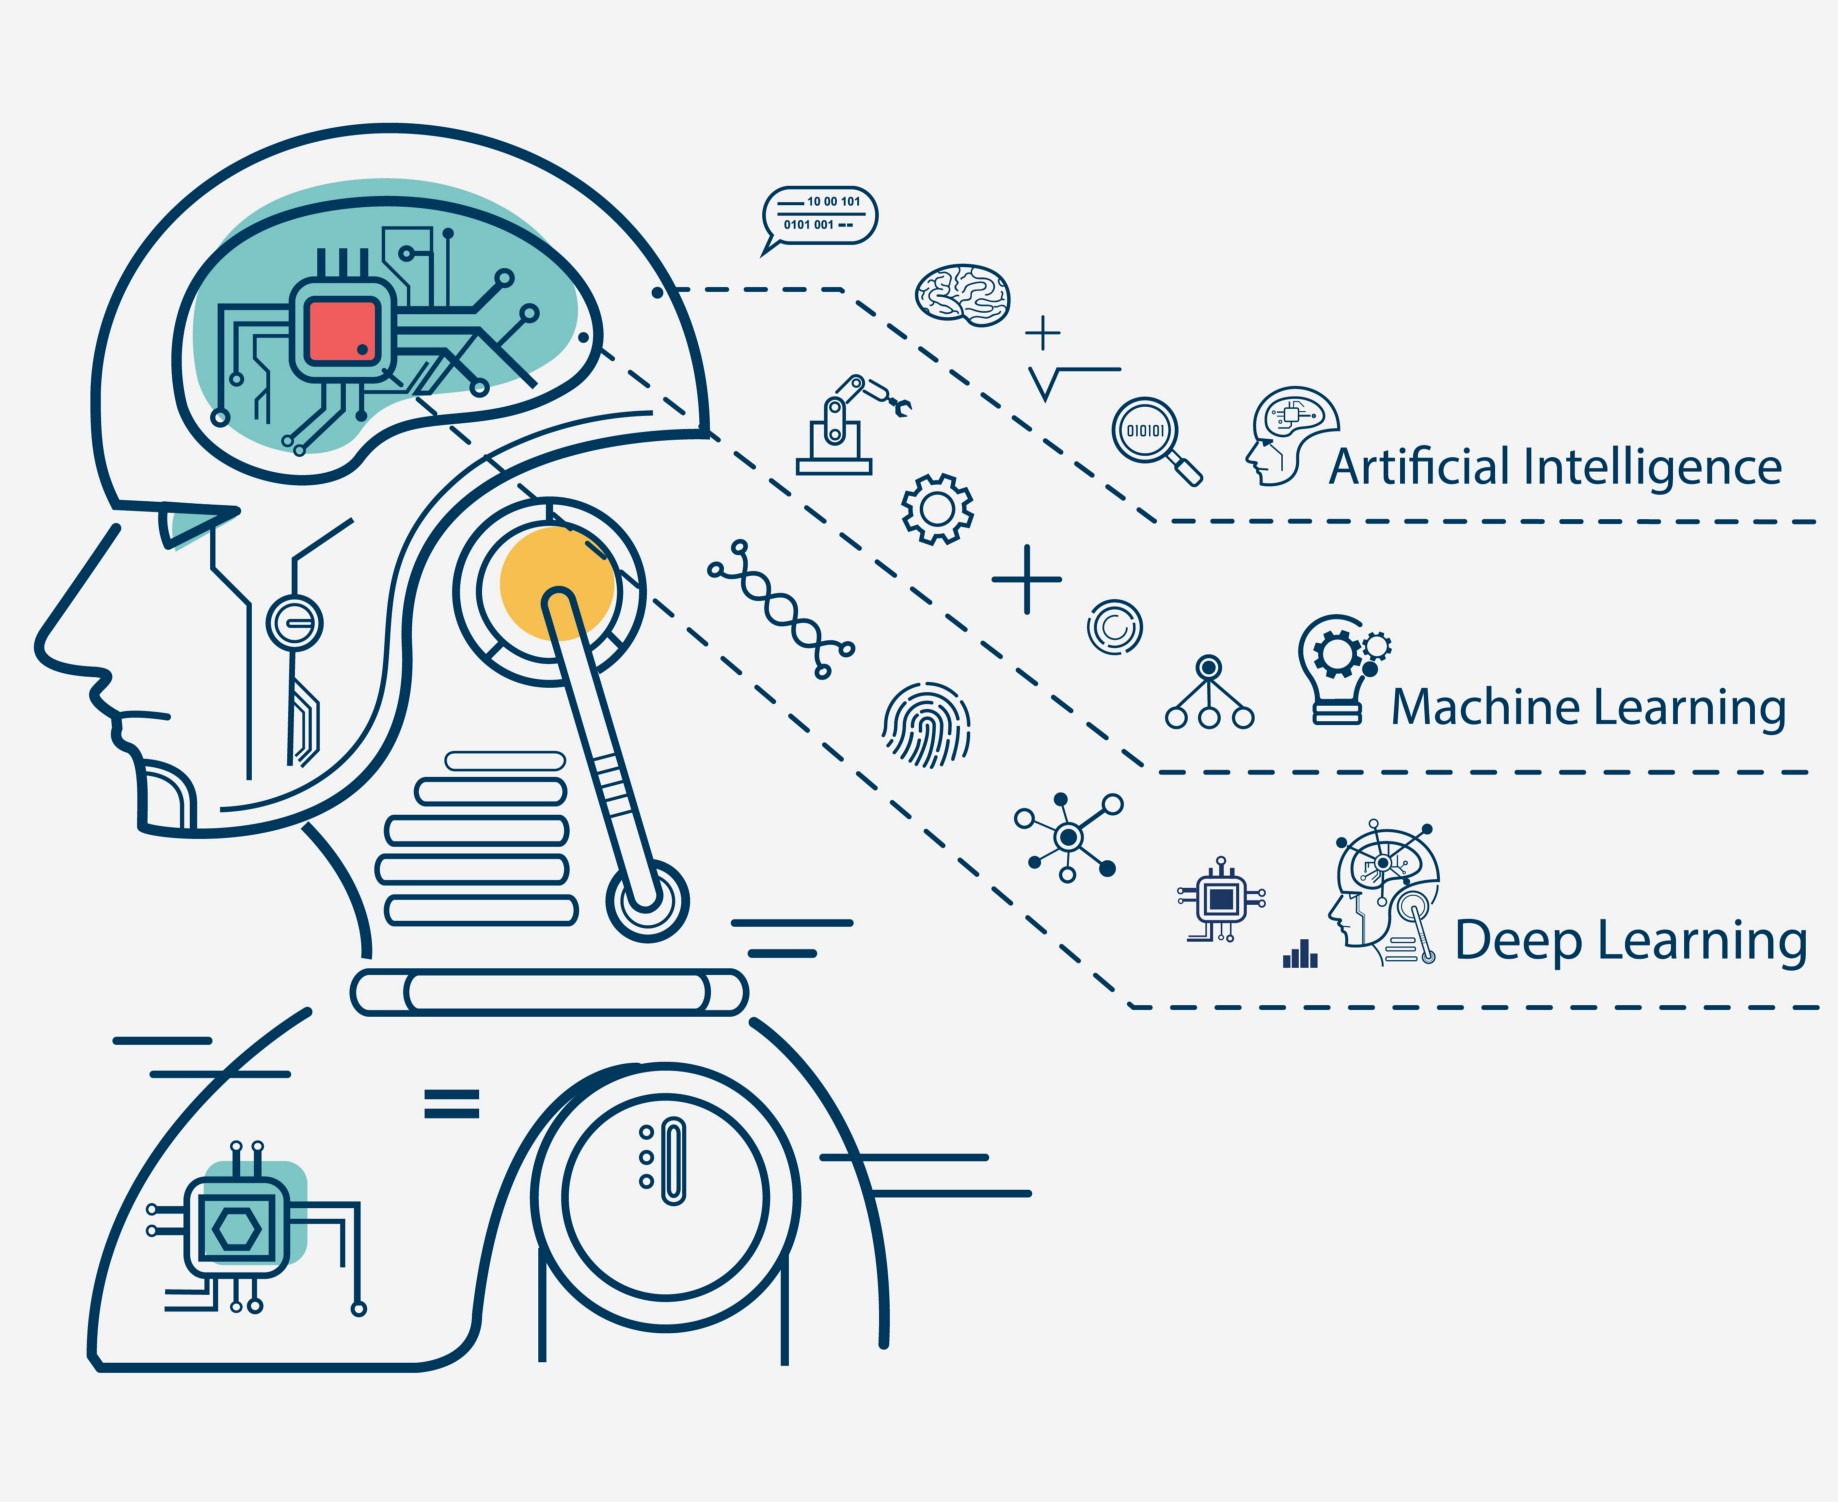
\includegraphics[width=\textwidth,height=.5\textheight]{imgs/intro.jpeg}}
%\usebackgroundtemplate{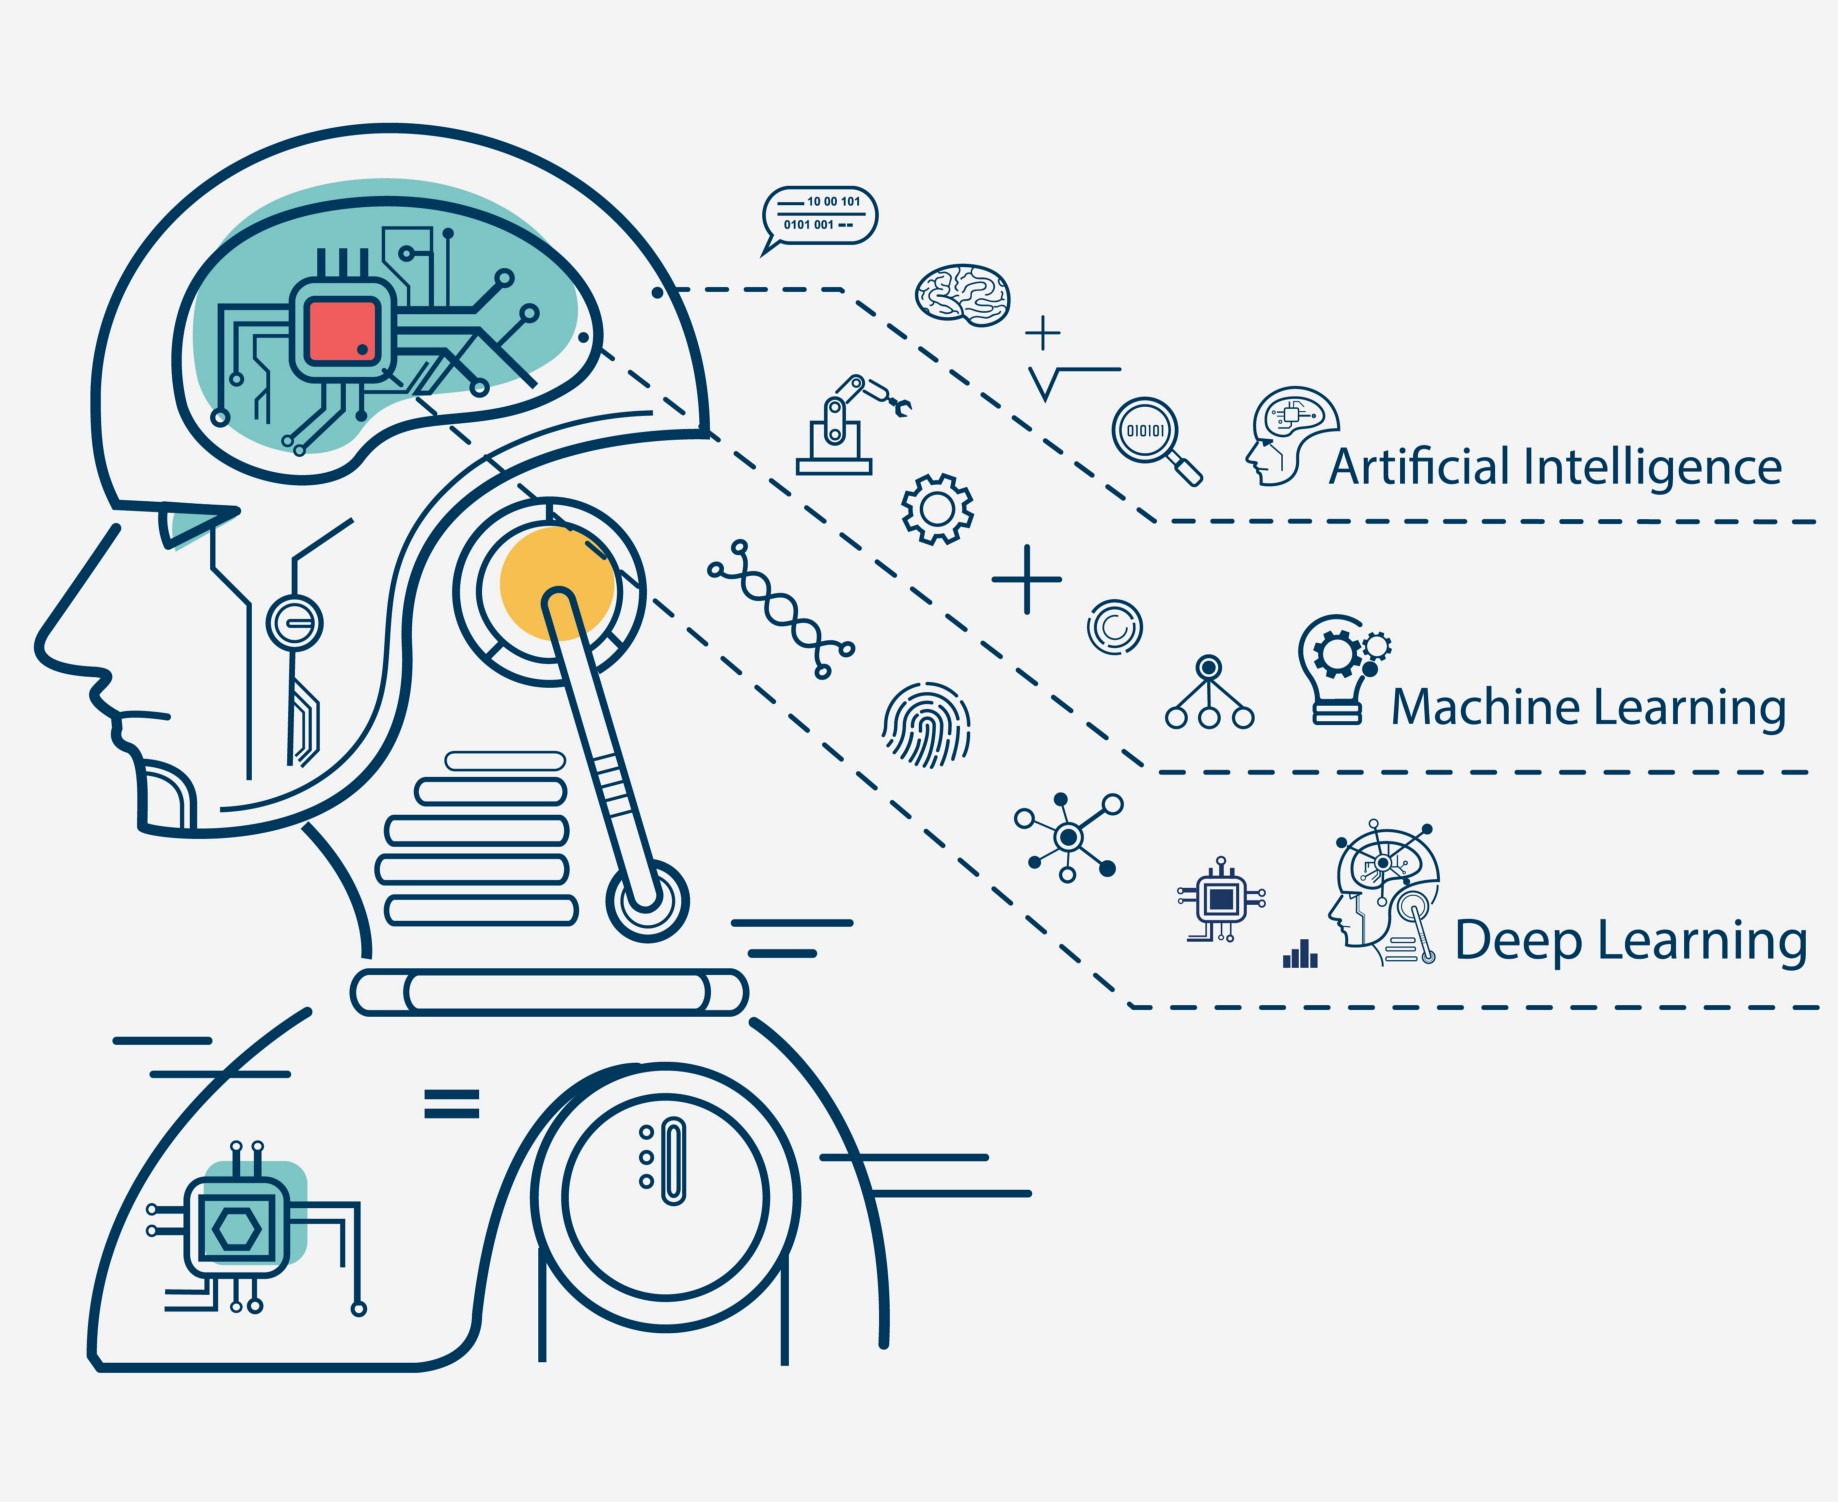
\includegraphics[width=\paperwidth]{imgs/intro.jpeg}}
\begin{document}

\begin{frame}[plain]
  \titlepage
\end{frame}

%
%\AtBeginSection[]
%{
%	\begin{frame}
%	\frametitle{Agenda}
%	\tableofcontents[currentsection]
%\end{frame}
%}


%%%%%%%%%%%%%%%%%%%%%%%%%%%%%%%%%%%%%%%%%%%%%%%%%%%%%%%%%%%%%%%%%%%%%%%%%%%%%%%%%%%%%%%%%%%%%%%%%%%%%%%%%%%%%%%%
%\section*{Roteiro}
%%%%%%%%%%%%%%%%%%%%%%%%%%%%%%%%%%%%%%%%%%%%%%%%%%%%%%%%%%%%%%%%%%%%%%%%%%%%%%%%%%%%%%%%%%%%%%%%%%%%%%%%%%%%%%%%
%
%\begin{frame}
%  \frametitle{Agenda}
%  \tableofcontents
%\end{frame}

%%%%%%%%%%%%%%%%%%%%%%%%%%%%%%%%%%%%%%%%%%%%%%%%%%%%%%%%%%%%%%%%%%%%%%%%%%%%%%%%%%%%%%%%%%%%%%%%%%%%%%%%%%%%%%%%
\section{Introdu��o}
%%%%%%%%%%%%%%%%%%%%%%%%%%%%%%%%%%%%%%%%%%%%%%%%%%%%%%%%%%%%%%%%%%%%%%%%%%%%%%%%%%%%%%%%%%%%%%%%%%%%%%%%%%%%%%%%

\begin{frame}{Introdu��o}{Data Augmentation}
\begin{itemize}
\item {\bf Data Augmentation} � uma t�cnica utilizada para artificialmente expandir a quantidade de dados usados para treinamento de um modelo.
\item Treinar modelos de {\it deep learning} utilizando mais dados pode resultar em maior acur�cia.
\item T�cnicas de {\it data augmentation} podem criar varia��es das imagens que tornam os modelos mais generalistas.
\end{itemize}

\vspace{2cm}
\tiny{Fonte: \href{https://towardsdatascience.com/simple-image-data-augmentation-technics-to-mitigate-overfitting-in-computer-vision-2a6966f51af4}{How to Configure Image Data Augmentation in Keras} }
\end{frame}

%%%%%%%%%%%%%%%%%%%%%%%%%%%%%%%%%%%%%%%%%%%%%%%%%%%%%%%%%%%%%%%%%%%%%%%%%%%%%%%%%%%%%%%%%%%%%%%%%%%%%%%%%%%%%%%%

\begin{frame}{Introdu��o}{Data Augmentation}
\begin{itemize}
\item Offline
\begin{itemize}
\item Realizada antes do treinamento do modelo.
\item Datasets pequenos.
\end{itemize}
\item Online ({\it augmentation on the fly})
\begin{itemize}
\item Executada em mini-batchs durante o treinamento.
\item Grandes datasets.
\end{itemize}
\end{itemize}

\vspace{1cm}
\tiny{Fonte: \href{https://nanonets.com/blog/data-augmentation-how-to-use-deep-learning-when-you-have-limited-data-part-2/}{Data Augmentation | How to use Deep Learning when you have Limited Data?} }
\end{frame}

%%%%%%%%%%%%%%%%%%%%%%%%%%%%%%%%%%%%%%%%%%%%%%%%%%%%%%%%%%%%%%%%%%%%%%%%%%%%%%%%%%%%%%%%%%%%%%%%%%%%%%%%%%%%%%%%

\begin{frame}{Data Augmentation}{Flip}
Flip Horizontal|Vertical
\begin{figure}[h]

\includegraphics[width=9cm]{imgs/data_aug_flip.png}
\end{figure}
\end{frame}

%%%%%%%%%%%%%%%%%%%%%%%%%%%%%%%%%%%%%%%%%%%%%%%%%%%%%%%%%%%%%%%%%%%%%%%%%%%%%%%%%%%%%%%%%%%%%%%%%%%%%%%%%%%%%%%%

\begin{frame}{Data Augmentation}{Rotation}
Rota��o de 90�
\begin{figure}[h]

\includegraphics[width=9cm]{imgs/data_aug_rotation.png}
\end{figure}
\end{frame}

%%%%%%%%%%%%%%%%%%%%%%%%%%%%%%%%%%%%%%%%%%%%%%%%%%%%%%%%%%%%%%%%%%%%%%%%%%%%%%%%%%%%%%%%%%%%%%%%%%%%%%%%%%%%%%%%

\begin{frame}{Data Augmentation}{Scale}
Scale=0,10\% | 20\%
\begin{figure}[h]

\includegraphics[width=9cm]{imgs/data_aug_scale.png}
\end{figure}
\end{frame}

%%%%%%%%%%%%%%%%%%%%%%%%%%%%%%%%%%%%%%%%%%%%%%%%%%%%%%%%%%%%%%%%%%%%%%%%%%%%%%%%%%%%%%%%%%%%%%%%%%%%%%%%%%%%%%%%

\begin{frame}{Data Augmentation}{Crop}
Crop top-left | bottom-right
\begin{figure}[h]

\includegraphics[width=9cm]{imgs/data_aug_crop.png}
\end{figure}
\end{frame}


%%%%%%%%%%%%%%%%%%%%%%%%%%%%%%%%%%%%%%%%%%%%%%%%%%%%%%%%%%%%%%%%%%%%%%%%%%%%%%%%%%%%%%%%%%%%%%%%%%%%%%%%%%%%%%%%

\begin{frame}{Data Augmentation}{Translation}
\begin{figure}[h]
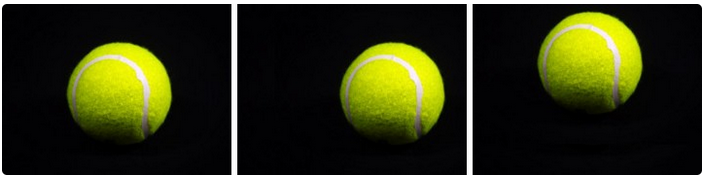
\includegraphics[width=9cm]{imgs/data_aug_translation.png}
\end{figure}
\end{frame}

%%%%%%%%%%%%%%%%%%%%%%%%%%%%%%%%%%%%%%%%%%%%%%%%%%%%%%%%%%%%%%%%%%%%%%%%%%%%%%%%%%%%%%%%%%%%%%%%%%%%%%%%%%%%%%%%

\begin{frame}{Data Augmentation}{Gaussian Noise}
\begin{figure}[h]
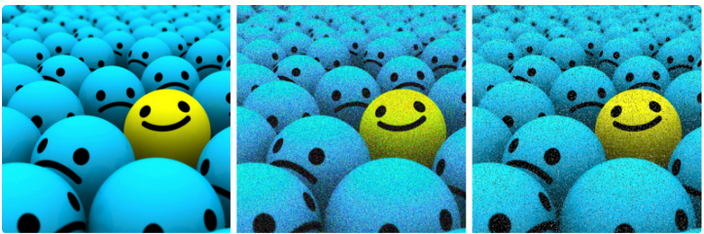
\includegraphics[width=9cm]{imgs/data_aug_gaussian_noise.png}
\end{figure}
\end{frame}


%%%%%%%%%%%%%%%%%%%%%%%%%%%%%%%%%%%%%%%%%%%%%%%%%%%%%%%%%%%%%%%%%%%%%%%%%%%%%%%%%%%%%%%%%%%%%%%%%%%%%%%%%%%%%%%%

\begin{frame}{Refer�ncias}
\begin{itemize}
\item Documentacao Oficial Tensorflow: Aumento de dados 
\begin{itemize}
\item \url{https://www.tensorflow.org/tutorials/images/data_augmentation}
\end{itemize}
\item How to Configure Image Data Augmentation in Keras
\begin{itemize}
\item \url{https://machinelearningmastery.com/how-to-configure-image-data-augmentation-when-training-deep-learning-neural-networks/}
\end{itemize}
\item Image Augmentation on the fly using Keras ImageDataGenerator!
\begin{itemize}
\item \url{https://www.analyticsvidhya.com/blog/2020/08/image-augmentation-on-the-fly-using-keras-imagedatagenerator/}
\end{itemize}
\end{itemize}
\end{frame}


%%%%%%%%%%%%%%%%%%%%%%%%%%%%%%%%%%%%%%%%%%%%%%%%%%%%%%%%%%%%%%%%%%%%%%%%%%%%%%%%%%%%%%%%%%%%%%%%%%%%%%%%%%%%%%%%

\begin{frame}[plain]
  \titlepage
\end{frame}



\end{document}
